\subsection{PSYCHE pure shift NMR}
\label{subsec:poise__psyche}

In \cref{sec:pureshift__optimisation}, I described the motivation behind, and early attempts towards, the optimisation of PSYCHE pure shift spectra.
The content in this section is similar, except that it was performed within the framework of POISE.

\begin{figure}[htb]
    \centering
    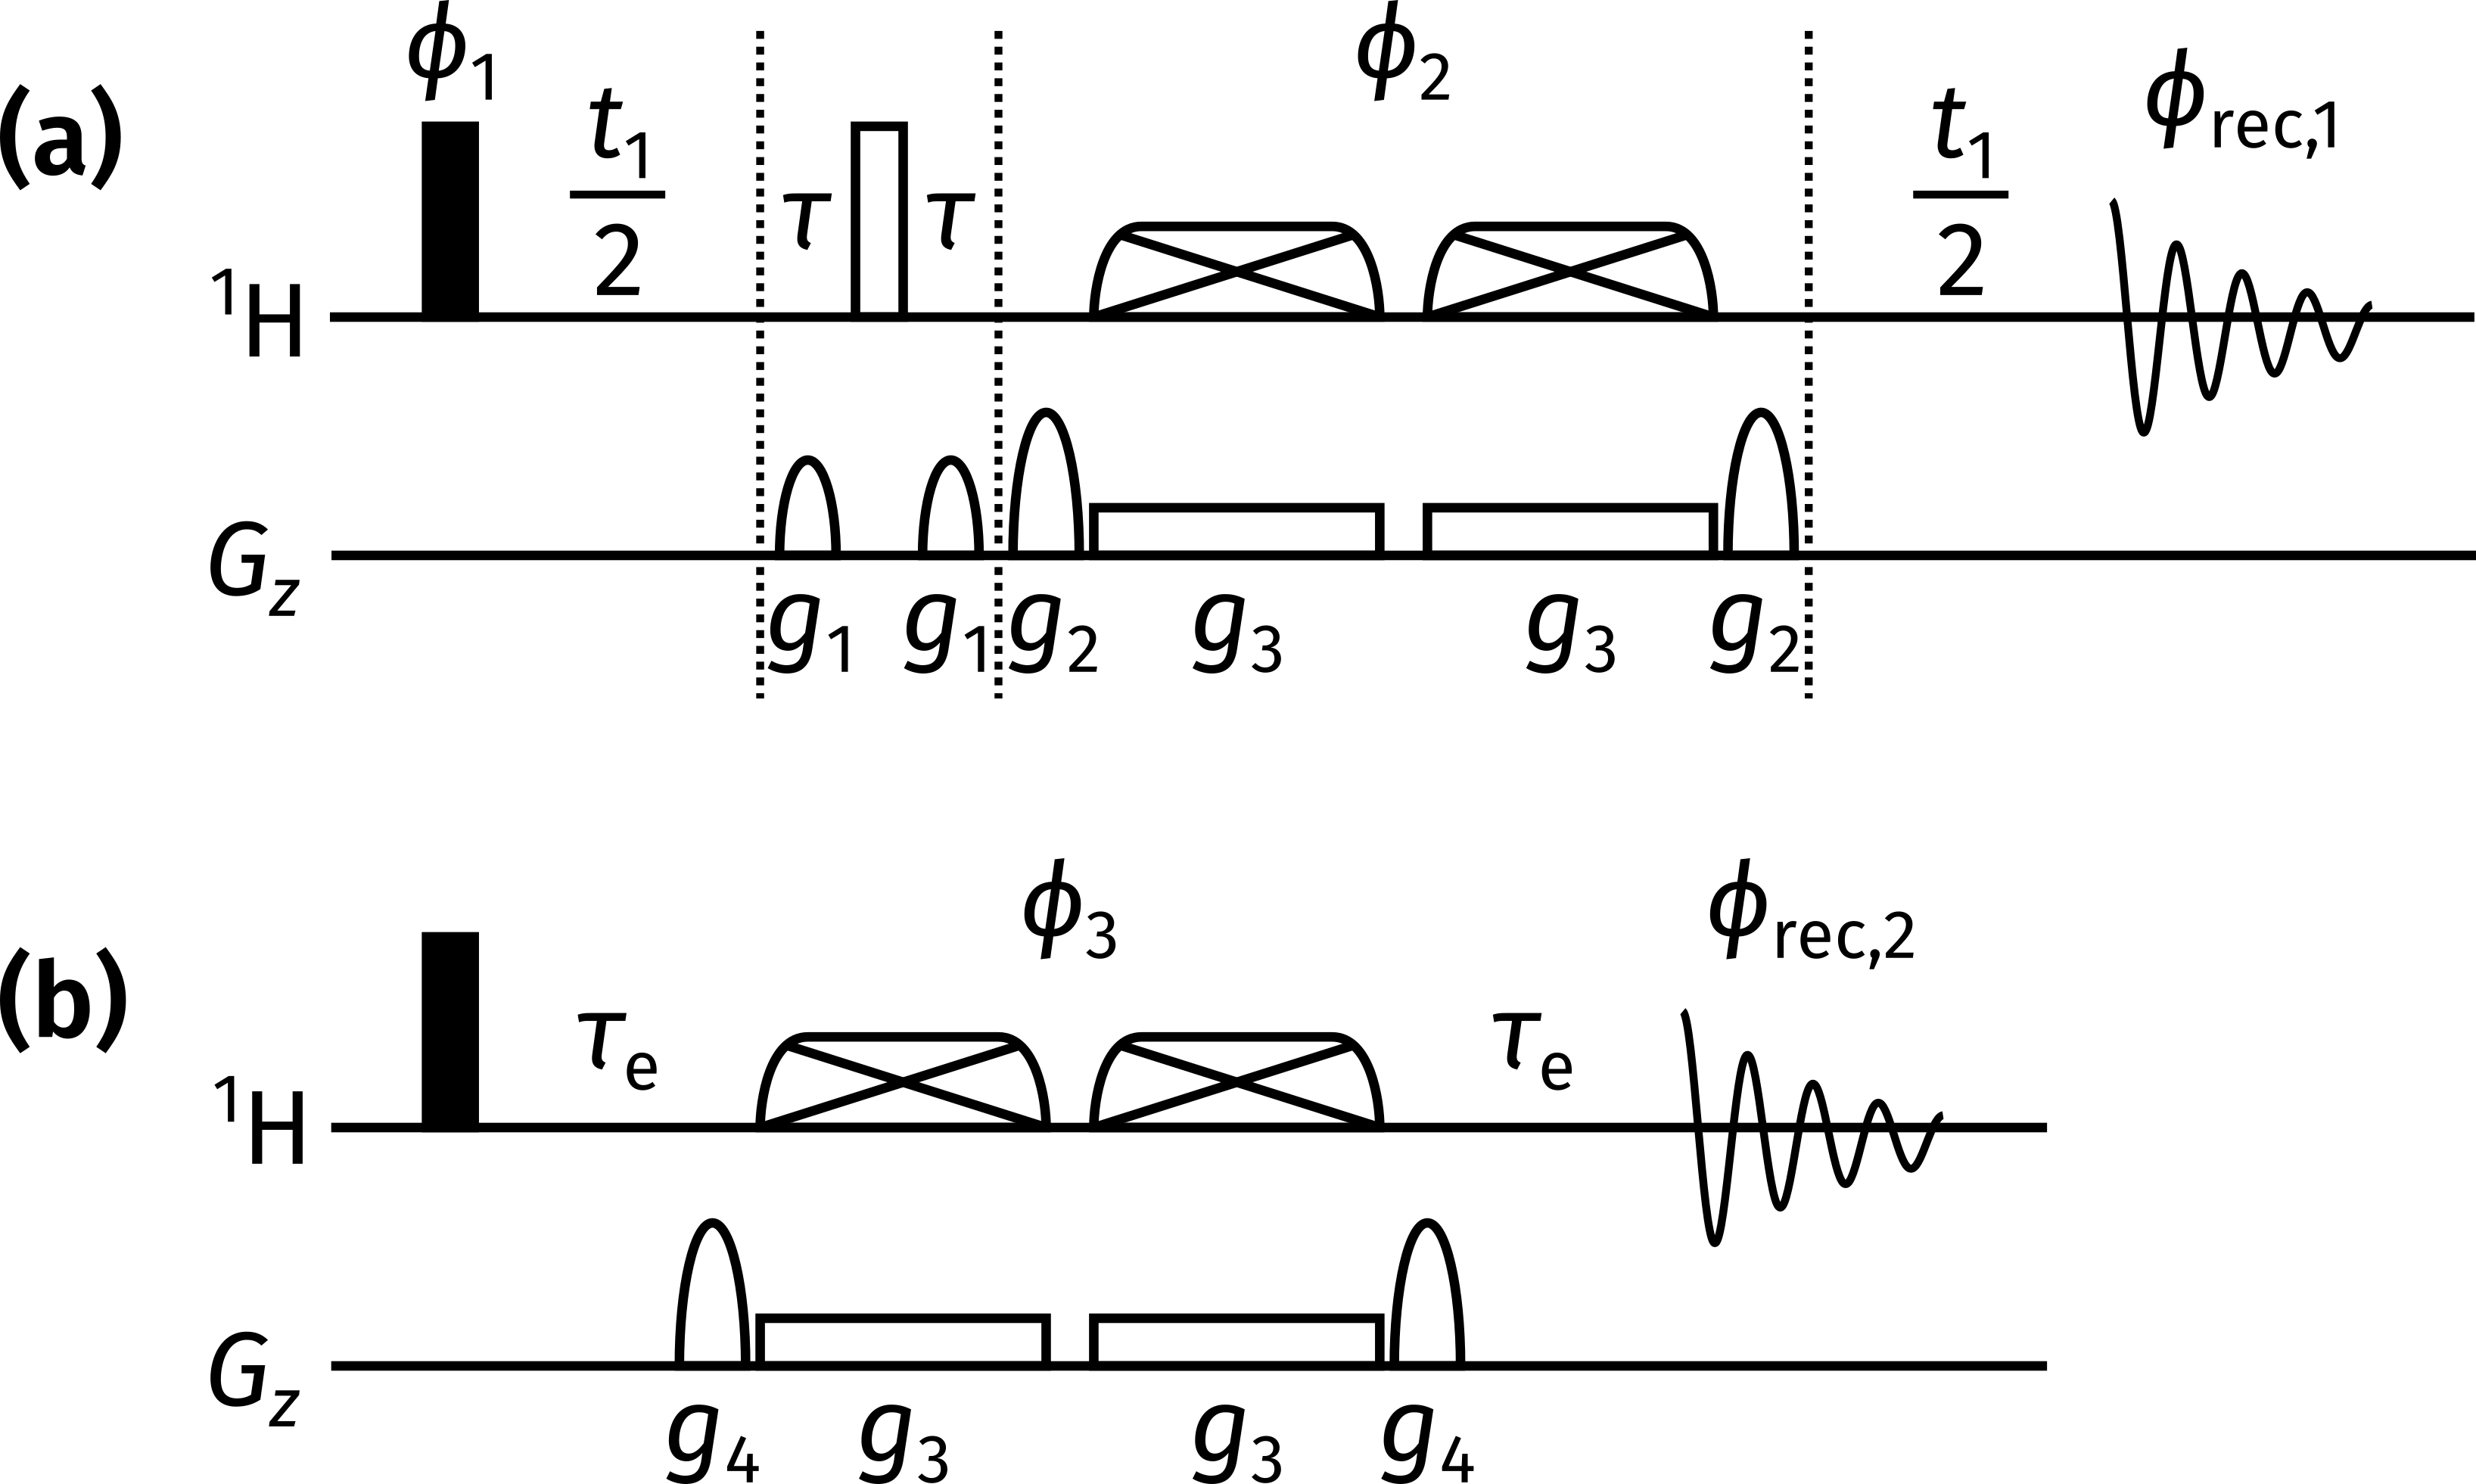
\includegraphics[]{pp/poise/psyche.png}%
    {\phantomsubcaption\label{fig:poise_psyche_pulseq_psyche}}%
    {\phantomsubcaption\label{fig:poise_psyche_pulseq_jrse}}%
    \caption[Pulse sequences used for PSYCHE optimisations]{
        \textbf{(\subref{fig:poise_psyche_pulseq_psyche})} Pseudo-2D PSYCHE pure shift experiment.
        \textbf{(\subref{fig:poise_psyche_pulseq_jrse})} J-resolved spin echo experiment (see also \cref{subsec:pureshift__optim_techniques}) using the PSYCHE PSE.
        Phase cycling is performed using: $\phi_1 = (x, -x)$, $\phi_2 = (x, x, y, y)$, $\phi_{\text{rec},1} = (x, -x, -x, x)$ for the full PSYCHE experiment, and $\phi_3 = (x, y, -x, -y)$, $\phi_{\text{rec},2} = (x, -x, x, -x)$ for the JRSE experiment.
        CTP gradient amplitudes are $(g_1, g_2, g_4) = (35\%, 77\%, 50\%)$ (though the exact values are likely immaterial); the PSYCHE gradient $g_3$ was subjected to optimisation.
        The delay $\tau$ is set to $1/(4 \cdot T_\text{chunk})$ for the PSYCHE experiment, and $\tau_\text{e}$ is \SI{16}{\ms}.
    }
    \label{fig:poise_psyche_pulseq}
\end{figure}



\subsubsection{Optimisation setup}

In this section, the standard double-saltire PSYCHE pure shift element was used (\cref{fig:poise_psyche_pulseq_psyche}).\autocite{Foroozandeh2014ACIE,Foroozandeh2018CEJ}
As described in \cref{subsec:pureshift__optim_techniques}, the PSYCHE pure shift element can be described using six parameters; in this section, we investigate only three of these, namely the amplitude (i.e.\ flip angle $\beta$), bandwidth $\Delta F$, and duration $\taup$.
In addition to this, the amplitude of the weak gradient during the PSE $g_3$ was also chosen as a fourth parameter to vary.
As before, the quality of the PSE is evaluated using a JRSE experiment (\cref{fig:poise_psyche_pulseq_jrse}), which is then compared against a pulse--acquire spectrum: the cost function used is $f_\text{diff}$.

In general, the spectral region being evaluated has to be appropriately chosen to exclude strong singlets, which are irrelevant to pure shift NMR but disproportionately influence the value of the cost function.
For the work in this chapter, which was performed on the andrographolide sample, the spectral region was therefore limited to \SI{1.15}{\ppm} and above.

In the JRSE pulse sequence used for optimisation, the four parameters (flip angle, bandwidth, duration, and gradient amplitude) are respectively \texttt{CNST20}, \texttt{CNST21}, \texttt{P40}, and \texttt{GPZ10}.
There is, however, a slight complication: whenever the bandwidth or duration is changed, the entire pulse must be re-created, because the $x$- and $y$-coefficients depend on these parameters.
Therefore, a (TopSpin) Python script was written to generate the double saltire pulse using the parameters above, and the POISE AU programme was modified to call this Python script before acquiring the spectrum.
Although the overall setup may perhaps be slightly confusing,%
\footnote{We have here a Python script (the POISE frontend) calling an AU programme (for acquisition) which calls a Python script (to make the double saltire).}
I contend that this is an excellent demonstration of the customisability that POISE provides.

One slightly odd behaviour noted with the PSYCHE optimisations was that at least one dummy scan was required for the optimisation to be robust:
if no dummy scans were used, the \textit{very first} FE in an optimisation run would yield a rather unreliable result, although subsequent FEs were unaffected.
It is not obvious why this is the case, as FEs are already separated by a delay of several seconds, on the order of $5T_1$: thus, each FE should be starting from (almost) full equilibrium magnetisation.
Nevertheless, all optimisations in this section were run using \texttt{DS=1} and \texttt{NS=2}.
The sample used was andrographolide: this is the same sample as was used in the dPSYCHE section (\cref{sec:pureshift__dpsyche}), and is useful for pure shift studies as it contains quite diverse coupling patterns.

\subsubsection{Optimisation results}

\begin{table}
    \centering
    \begin{tabular}{cccccccc}
        \toprule
         & \multicolumn{3}{c}{Aggregated results from all runs} & \multicolumn{4}{c}{Parameters from best optimum} \\
        \cmidrule(lr){2-4} \cmidrule(lr){5-8}
        Description & $f_\mathrm{diff}$ & FEs              & Time (\si{\s}) & $\beta$ ($^\circ$) & $g_3$ (\%) & $\Delta F$ (kHz) & $\tau_\mathrm{p}$ (ms) \\
        \midrule
        Initial point & 0.353        & --     & --        & (25.0) & (2.00) & (10.0) & (30.0) \\
        1 parameter   & 0.340--0.343 & 5--10  & 84--168   & 17.5   & (2.00) & (10.0) & (30.0) \\
        2 parameters  & 0.325--0.338 & 12--33 & 205--565  & 16.5   & 1.00   & (10.0) & (30.0) \\
        3 parameters  & 0.320--0.328 & 18--77 & 315--1344 & 17.4   & 1.73   & 15.9   & (30.0) \\
        4 parameters  & 0.316--0.333 & 39--85 & 705--1504 & 13.9   & 1.45   & 15.9   & 36.0   \\
        \bottomrule
    \end{tabular}
    \caption[Overview of all PSYCHE optimisations]{
        Summary of all optimisations performed on the PSYCHE PSE.
        Unlike before, aggregated results are not grouped by optimisation algorithm; these ranges are therefore collected from a total of 15 runs (5 per algorithm).
        Parameters in parentheses were not optimised and were simply carried over from the initial point.
        A detailed breakdown of the results by algorithm, as well as the POISE routines used, are described in \cref{tbl:poise_psyche1p,tbl:poise_psyche2p,tbl:poise_psyche3p,tbl:poise_psyche4p}.
        \datacode{6A-200822}
    }
    \label{tbl:poise_psyche_summary}
\end{table}

\begin{figure}[htb]
    \centering
    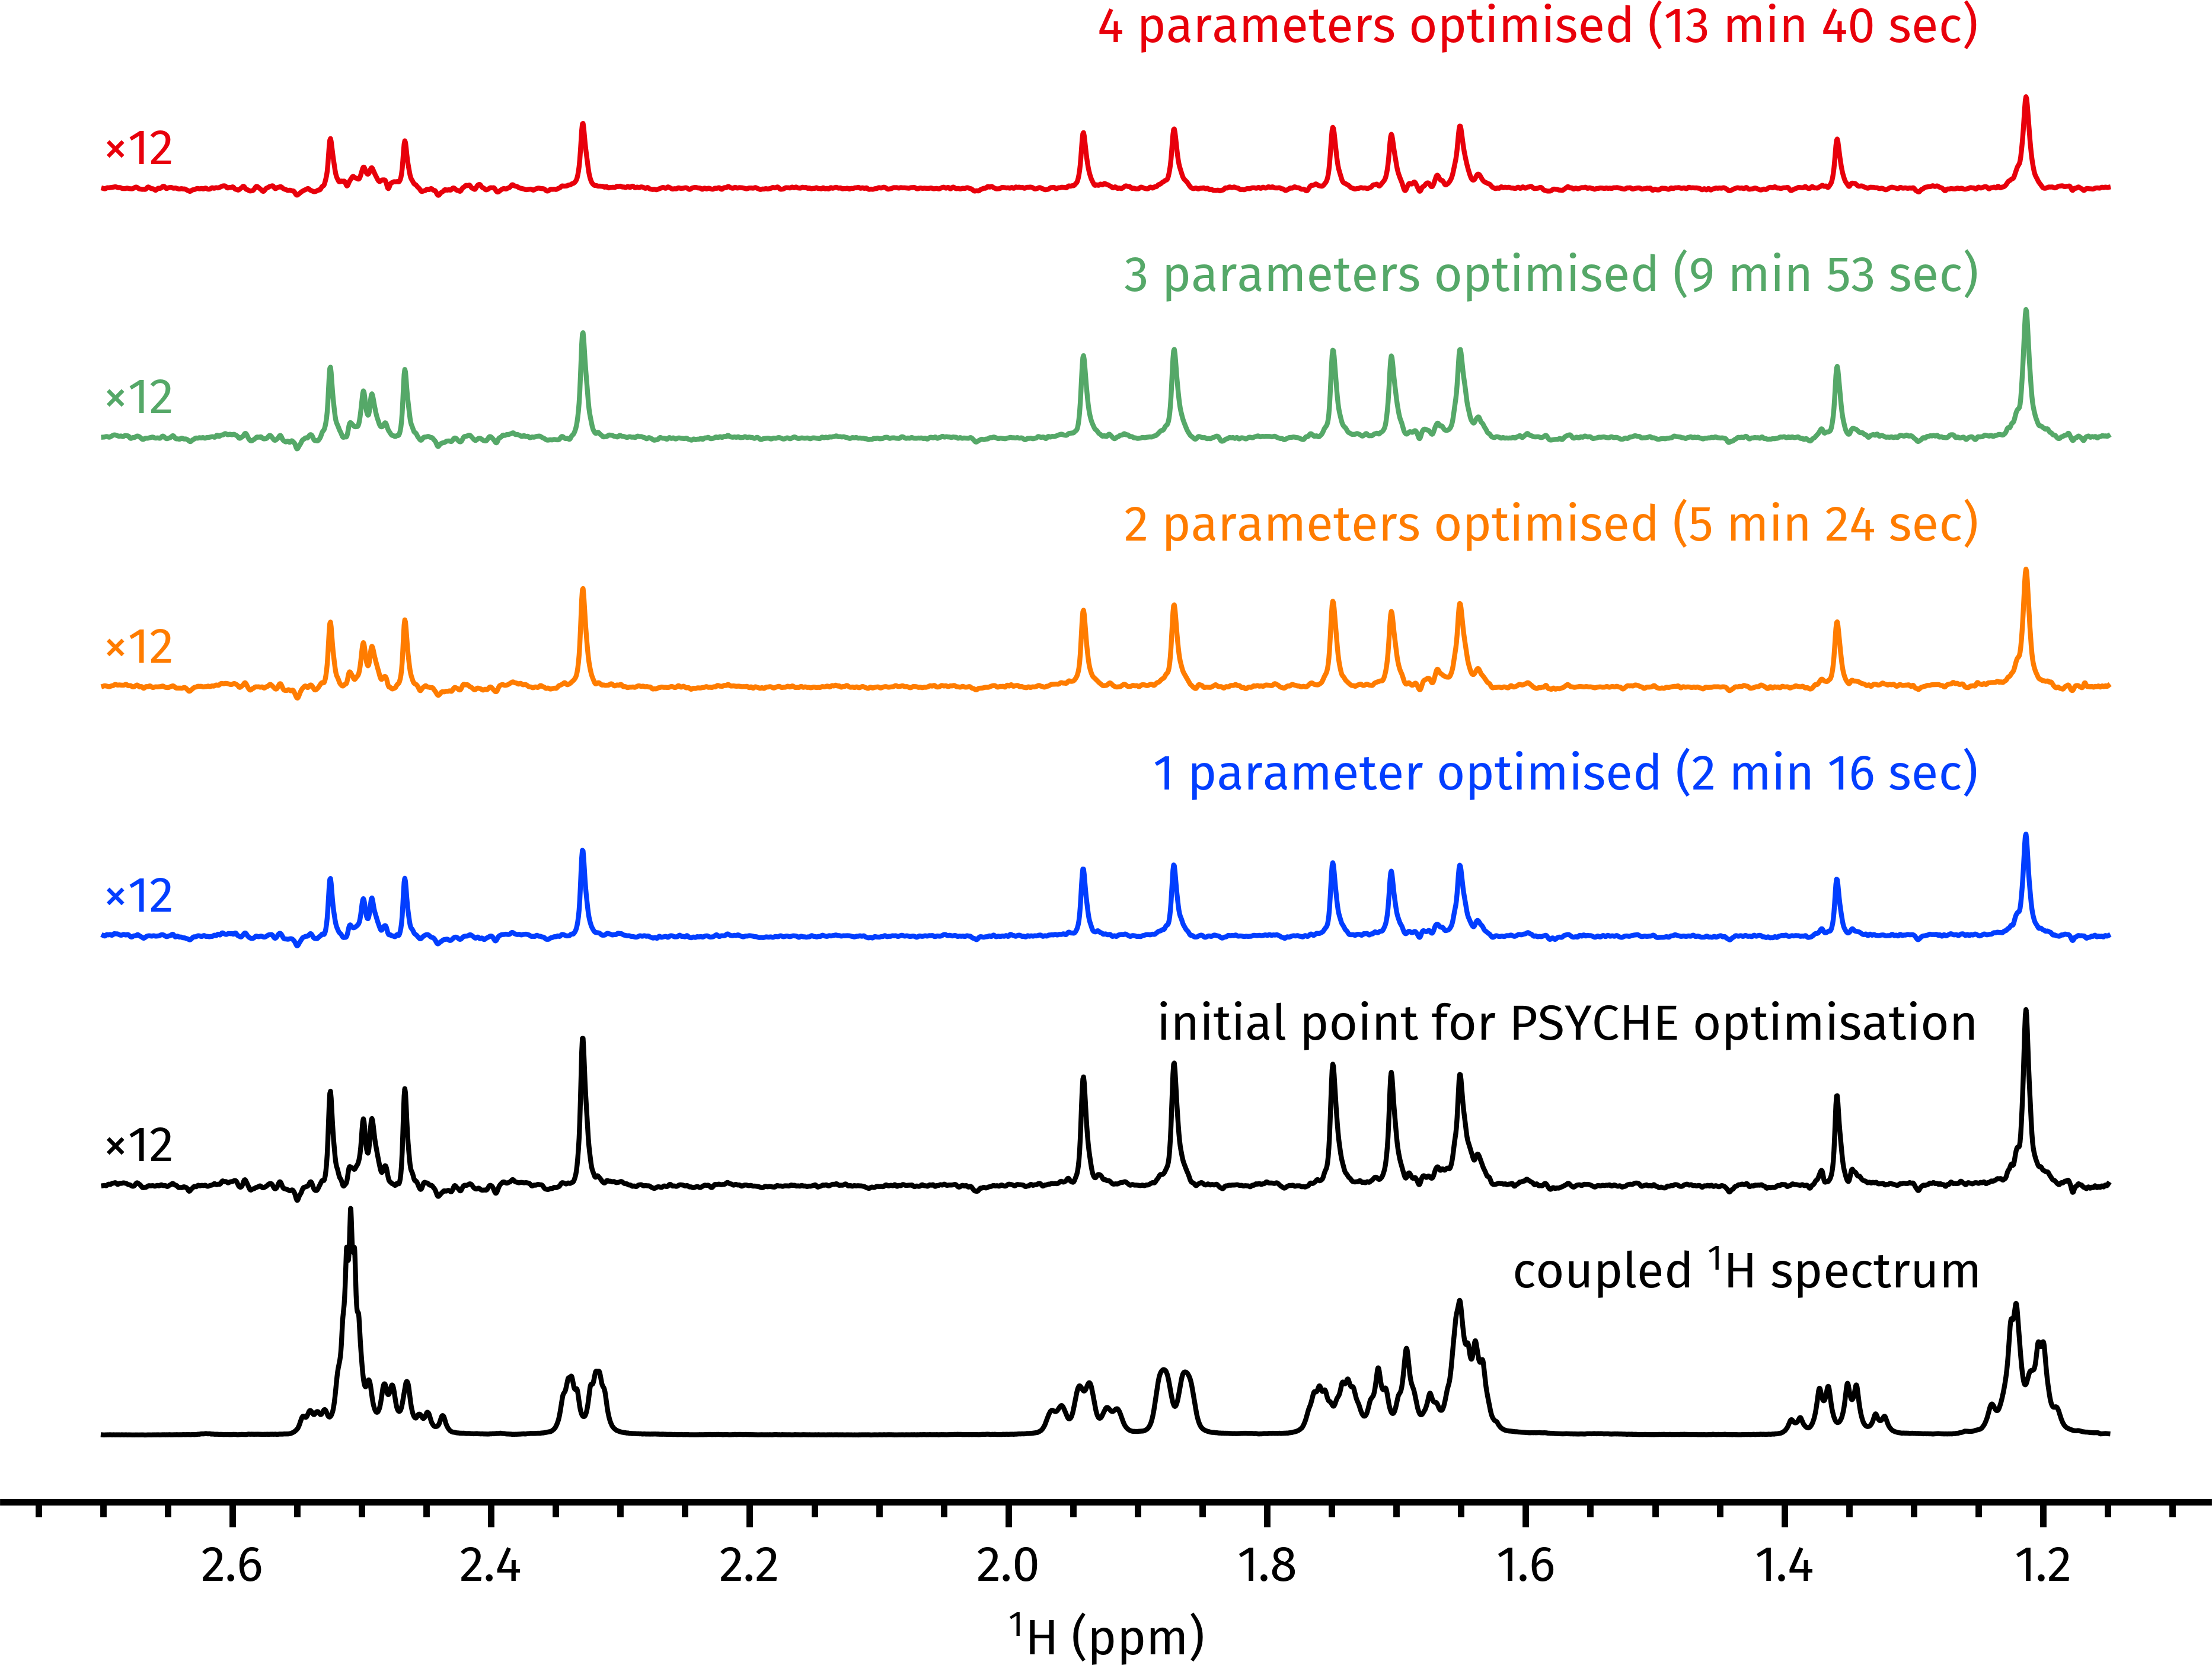
\includegraphics[draft=false]{poise/psyche_spec.png}%
    \caption[PSYCHE spectra before and after optimisation]{
        Insets of PSYCHE spectra obtained using the best optimum from each set of optimisations in \cref{tbl:poise_psyche_summary}; the time required to obtain the optimised parameters is also indicated for each spectrum.
        The original coupled \proton{} spectrum is shown as a reference.
        \datacode{6A-200823}
    }
    \label{fig:poise_psyche_spec}
\end{figure}

I ran several different optimisations of increasing complexity:
\begin{itemize}
    \item 1-parameter: flip angle only
    \item 2-parameter: flip angle and gradient amplitude
    \item 3-parameter: flip angle, gradient amplitude, and bandwidth
    \item 4-parameter: flip angle, gradient amplitude, bandwidth, and duration
\end{itemize}

\Cref{tbl:poise_psyche_summary} summarises the results obtained from all optimisations, whereas \cref{tbl:poise_psyche1p,tbl:poise_psyche2p,tbl:poise_psyche3p,tbl:poise_psyche4p} shows more detailed results for each individual set of optimisations, including a breakdown by algorithm.
We can see from these results that---perhaps unsurprisingly---optimising more parameters leads to greater improvements in the cost function, albeit at the cost of more FEs and more time.

An important question is whether these reductions in the cost function (measured on a JRSE experiment) do actually translate into improved pure shift spectra.
The pure shift spectra obtained with the optimised parameters in \cref{tbl:poise_psyche_summary} are shown in \cref{fig:poise_psyche_spec}.
Of particular interest are the two strongly coupled protons at \SI{2.5}{\ppm}: in the pure shift spectrum, the two peaks on either side are genuine, but strong coupling artefacts appear in the middle of these peaks.
On top of that, the decoupling performance for the peaks at \SI{1.36}{\ppm} and \SI{1.65}{\ppm} are also worth noting.

Broadly speaking, all the optimised spectra provide better performance than the initial point in terms of decoupling quality.
In particular, the 4-parameter optimisation successfully suppresses some of the strong coupling artefacts: this may be explained by the fact that the pulse duration was increased from \SI{30}{\ms} to \SI{36}{\ms}, which generally results in better spatiotemporal averaging, as was noted in \cref{sec:pureshift__nsaltire}.%
\footnote{This does raise the question of whether a two-parameter optimisation of just the flip angle and duration could yield similar results, but in a shorter time. I think it is possible, but I did not test this, though, as I simply did not have the appetite to try optimising \textit{every} possible combination of parameters.}
Generally, this optimisation \textit{does} come at a cost in sensitivity, which is especially obvious for the 4-parameter optimised result.
However, since the cost function $f_\text{diff}$ also penalises sensitivity losses, it also ensures that any drops in sensitivity are not excessive.

Given these improvements, one might wonder why it would ever be worth optimising fewer than four parameters.
The first obvious drawback is the time required: in fact, it is probably more economical to use the TSE-PSYCHE experiment (which also has improved performance in the presence of strong coupling).%
\footnote{Another thing I did not (thoroughly) investigate was to optimise the TSE-PSYCHE experiment. This could, in principle, be done using a TSE form of the JRSE experiment: \ang{90}--chirp--$\tau$--PSE--chirp--$\tau$--detect. However, this has decreased sensitivity over the original JRSE experiment, which means even longer optimisations.}
Furthermore, that $f_\text{diff}$ is a rather `flat' cost function and optimisations using it are very susceptible to noise: this factor is specific to pure shift optimisations, and was previously mentioned in \cref{subsec:pureshift__chirpopt}.
A closer inspection of the POISE logs for the 3- and 4-parameter optimisations (which are not provided here, but can be accessed in the raw data for the POISE paper which I uploaded at \url{https://doi.org/10.5281/zenodo.4698423}) reveals that the optimisations are perhaps not as consistent as one would hope.
Although \textit{generally} the optimisation leads to similar results in that (for example) $\beta$ is often decreased and $\taup$ increased, the extents of these changes are not quite uniform: for example, $\taup$ is optimised to anywhere between \SI{36}{\ms} and \SI{55}{\ms}, which suggests that there are \textit{many} local minima and which of these the optimisation converges to depends on the noise in the cost function.%
\footnote{I still think, however, that it is misleading to quote these ranges in \cref{tbl:poise_psyche1p,tbl:poise_psyche2p,tbl:poise_psyche3p,tbl:poise_psyche4p}, because this gives the impression that there are no correlations between the optimised parameters.}

Putting all of these factors together, it is (in my opinion) only really worthwhile to optimise two parameters at a time: either the flip angle plus gradient amplitude, or the flip angle plus the duration, appear to be sensible choices.
That said, this \textit{does} demonstrate that optimising multiple parameters at once---ordinarily a very challenging task for a human---does not actually require prohibitively long times when performed using a suitable algorithm.

\begin{table}
    \hbadness=10000
    \centering
    \begin{tabular}{ccccc}
        \toprule
       Entry & Algorithm & Optimum found (\si{\degree}) & FEs   & Time (\si{\s}) \\
        \midrule
        1     & NM        & 15.0--20.0                   & 8--10 & 135--168             \\
        2     & MDS       & 17.5--20.0                   & 8     & 133--136             \\
        3     & BOBYQA    & 18.4--19.9                   & 5     & 84--85               \\
        \bottomrule
    \end{tabular}
    \caption[PSYCHE 1-parameter optimisations]{
        PSYCHE 1-parameter (flip angle) optimisations.
        The POISE routine used was: \mintinline[breaklines]{json}{{"name": "psyche1", "pars": ["cnst20"], "lb": [10.0], "ub": [35.0], "init": [25.0], "tol": [2.0], "cf": "specdiff", "au": "poise_1d"}}.
        \datacode{6A-200822}
    }
    \label{tbl:poise_psyche1p}
\end{table}

\begin{table}
    \hbadness=10000
    \centering
    \begin{tabular}{ccccccc}
        \toprule
              &           & \multicolumn{3}{c}{Best optimum found}            & \multicolumn{2}{c}{Aggregated results} \\
                            \cmidrule(lr){3-5}                                  \cmidrule(lr){6-7}
        Entry & Algorithm & $\beta$ ($^\circ$) & $g_3$ (\%) & $f_\text{diff}$ & FEs    & Time (\si{\s}) \\
        \midrule
        1     & NM        & 16.48              & 1.00       & 0.3253          & 18--24 & 307--410             \\
        2     & MDS       & 18.47              & 0.82       & 0.3261          & 25--33 & 424--565             \\
        3     & BOBYQA    & 15.77              & 0.96       & 0.3279          & 12--16 & 205--271             \\
        \bottomrule
    \end{tabular}
    \caption[PSYCHE 2-parameter optimisations]{
        PSYCHE 2-parameter (flip angle and gradient amplitude) optimisations.
        The POISE routine used was: \mintinline[breaklines]{json}{{"name": "psyche2", "pars": ["cnst20", "gpz10"], "lb": [10.0, 0.2], "ub": [35.0, 5.0], "init": [25.0, 2.0], "tol": [2.0, 0.2], "cf": "specdiff", "au": "poise_1d"}}.
        \datacode{6A-200822}
    }
    \label{tbl:poise_psyche2p}
\end{table}

\begin{table}
    \hbadness=10000
    \centering
    \begin{tabular}{cccccccc}
        \toprule
              &           & \multicolumn{4}{c}{Best optimum found} & \multicolumn{2}{c}{Aggregated results} \\
                            \cmidrule(lr){3-6}                     \cmidrule(lr){7-8}
        Entry & Algorithm & $\beta$ ($^\circ$) & $g_3$ (\%) & $\Delta F$ (\si{\kHz}) & $f_\text{diff}$ & FEs    & Time (\si{\s}) \\
        \midrule
        1     & NM        & 17.40              & 1.73       & 15.93                  & 0.3196          & 33--43 & 576--770             \\
        2     & MDS       & 16.75              & 1.71       & 16.33                  & 0.3215          & 46--77 & 804--1344            \\
        3     & BOBYQA    & 16.48              & 1.65       & 16.71                  & 0.3200          & 18--31 & 315--540             \\
        \bottomrule
    \end{tabular}
    \caption[PSYCHE 3-parameter optimisations]{
        PSYCHE 3-parameter (flip angle, gradient amplitude, and bandwidth) optimisations.
        The POISE routine used was: \mintinline[breaklines]{json}{{"name": "psyche3", "pars": ["cnst20", "gpz10", "cnst21"], "lb": [10.0, 0.2, 1000.0], "ub": [35.0, 5.0, 20000.0], "init": [25.0, 2.0, 10000.0], "tol": [2.0, 0.2, 500.0], "cf": "specdiff", "au": "poise_psyche"}}.
        \datacode{6A-200822}
    }
    \label{tbl:poise_psyche3p}
\end{table}

\begin{table}
    \hbadness=10000
    \centering
    \begin{tabular}{ccccccccc}
        \toprule
              &           & \multicolumn{5}{c}{Best optimum found} & \multicolumn{2}{c}{Aggregated results} \\
                            \cmidrule(lr){3-7}                       \cmidrule(lr){8-9}
        Entry & Algorithm & $\beta$ ($^\circ$) & $g_3$ (\%) & $\Delta F$ (\si{\kHz}) & $\taup$ (\si{\ms}) & $f_\text{diff}$ & FEs    & Time (\si{\s}) \\
        \midrule
        1     & NM        & 13.87              & 1.45       & 15.93                  & 36.00              & 0.3163          & 40--47 & 733--845       \\
        2     & MDS       & 19.15              & 1.06       & 11.19                  & 36.52              & 0.3185          & 57--85 & 1006--1504     \\
        3     & BOBYQA    & 17.59              & 1.20       & 12.76                  & 43.06              & 0.3178          & 39--62 & 705--1130      \\
        \bottomrule
    \end{tabular}
    \caption[PSYCHE 4-parameter optimisations]{
        PSYCHE 4-parameter (flip angle, gradient amplitude, bandwidth, and pulse duration) optimisations.
        The POISE routine used was: \mintinline[breaklines]{json}{{"name": "psyche4", "pars": ["cnst20", "gpz10", "cnst21", "p40"], "lb": [10.0, 0.2, 1000.0, 5000.0], "ub": [35.0, 5.0, 20000.0, 75000.0], "init": [25.0, 2.0, 10000.0, 30000.0], "tol": [2.0, 0.2, 500.0, 2000.0], "cf": "specdiff", "au": "poise_psyche"}}.
        \datacode{6A-200822}
    }
    \label{tbl:poise_psyche4p}
\end{table}
